\subsection{Runtime view}

The main runtime interaction between the components of the system are briefly described and shown through the use of sequence diagrams.

\paragraph{User registration}

\begin{figure}[H]
	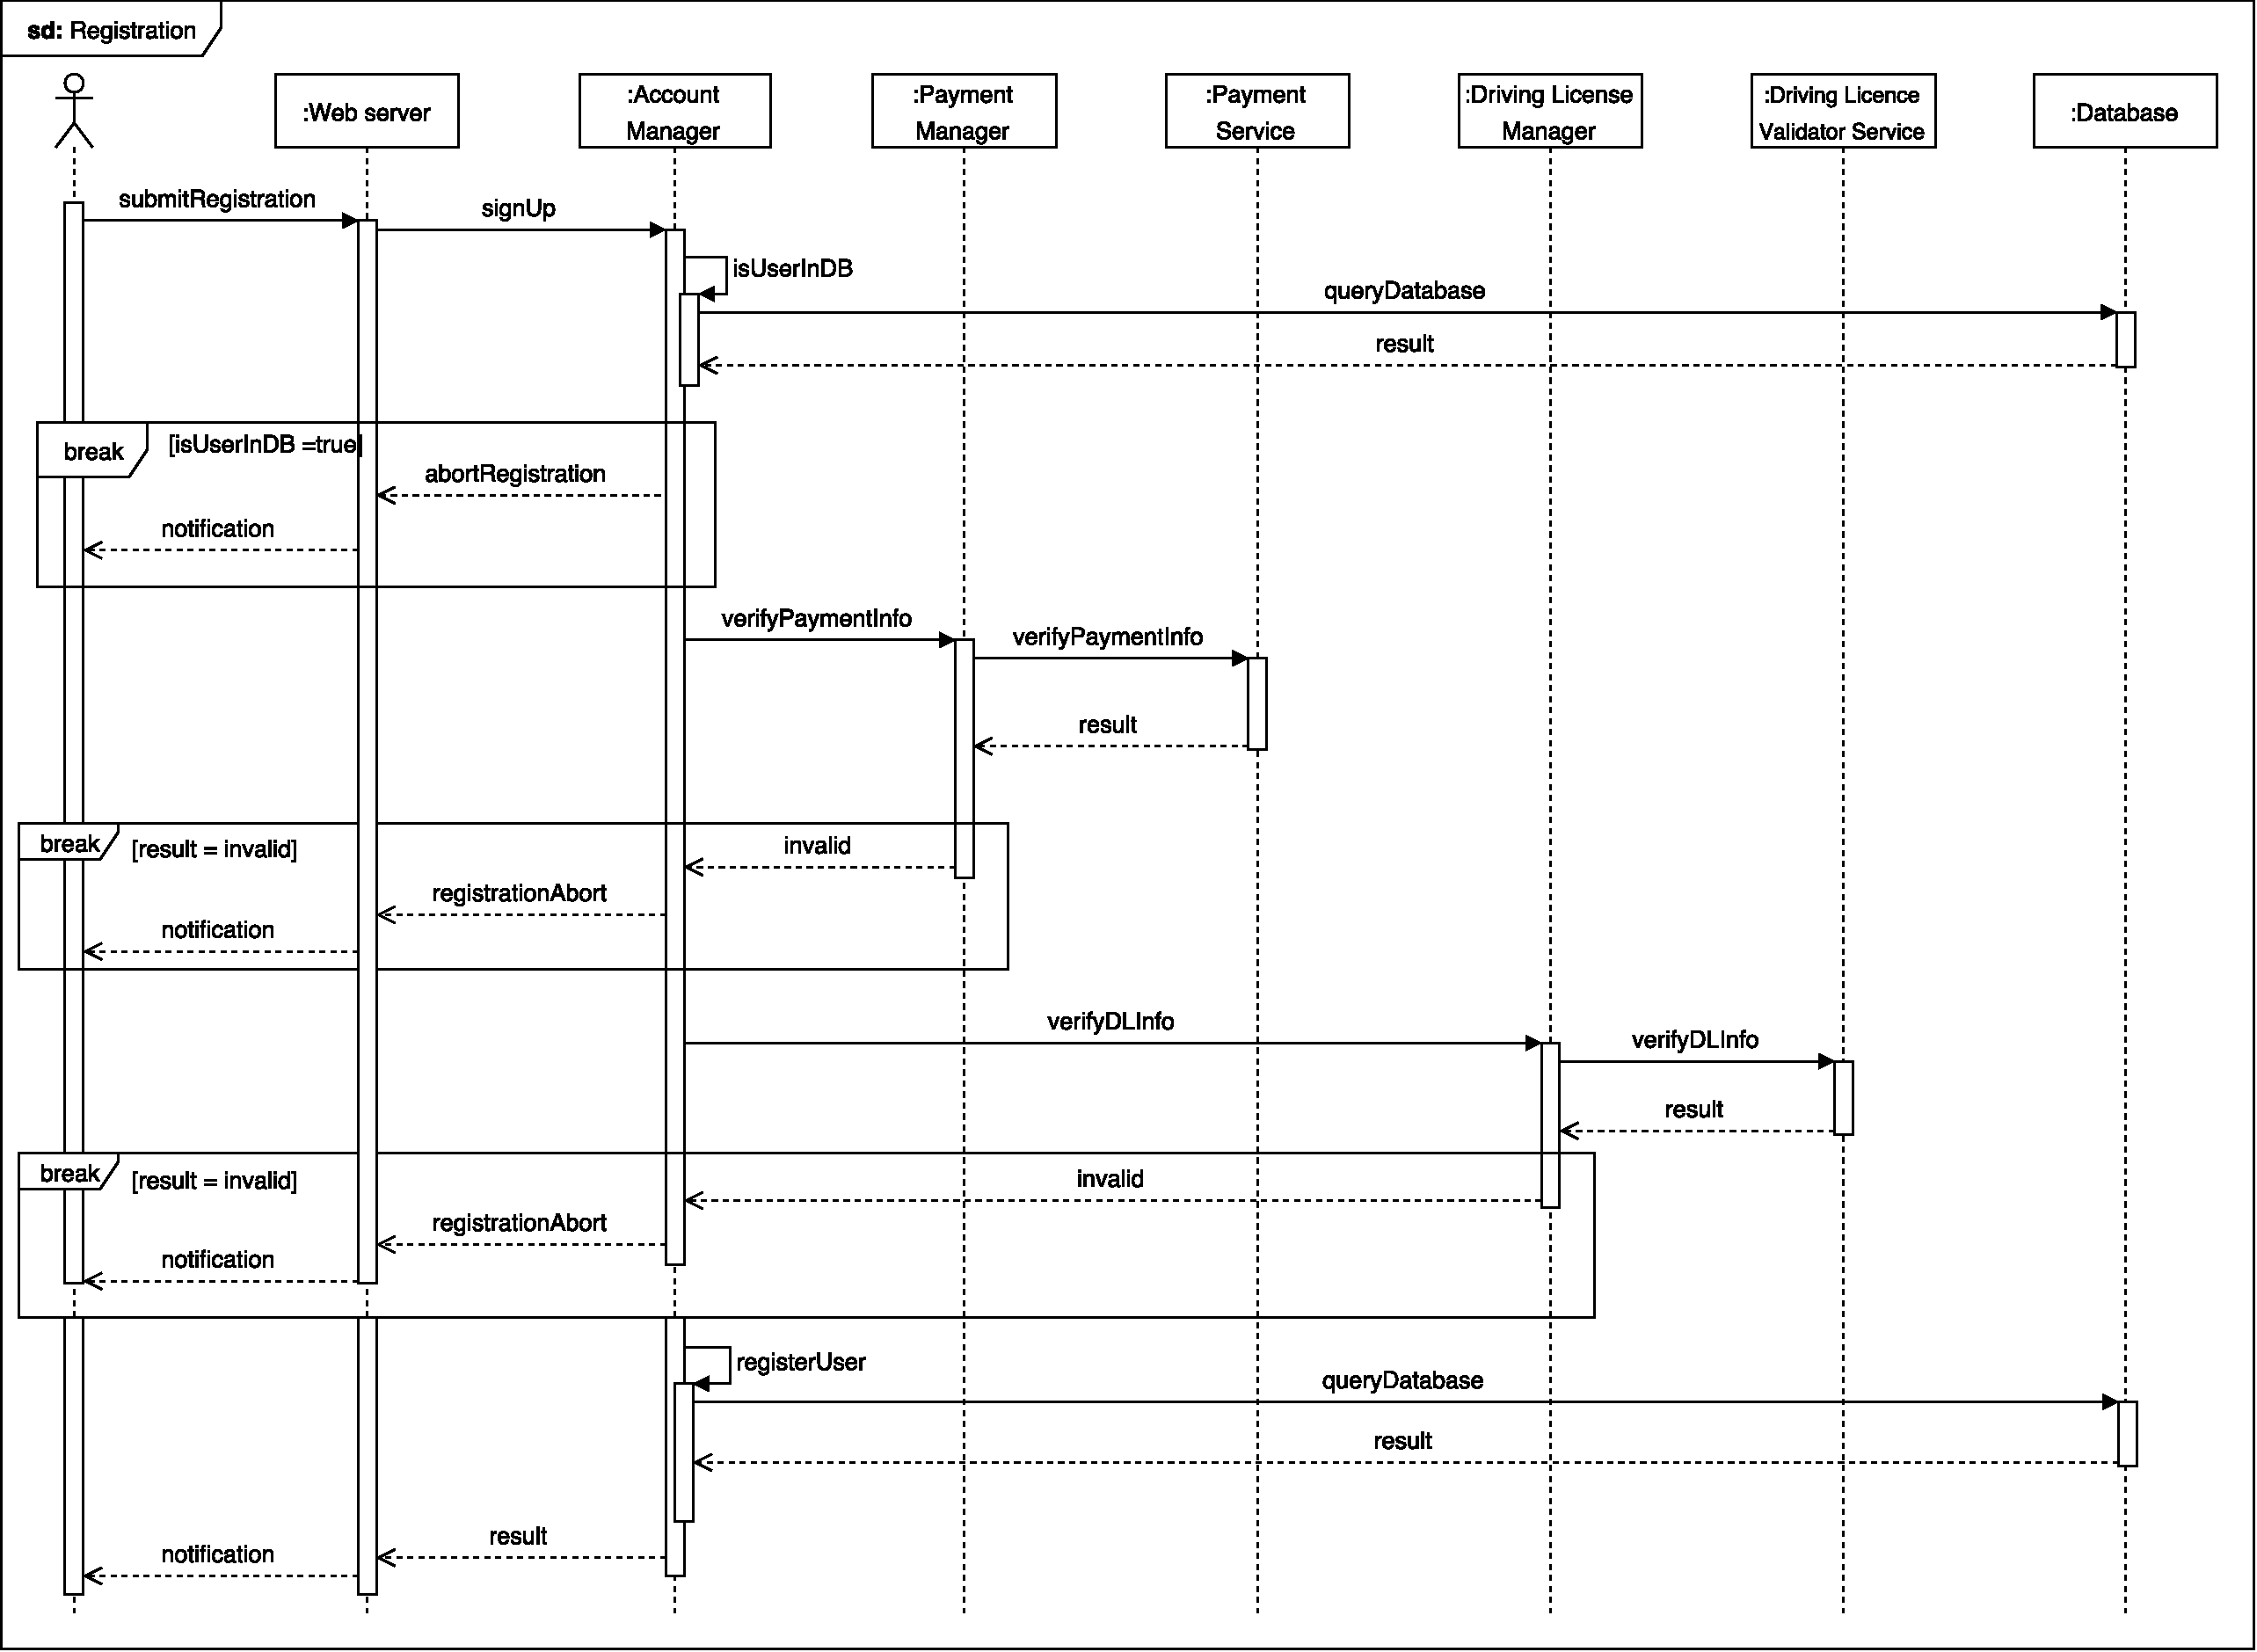
\includegraphics[width=350px]{../Datas/diagrams/registration.pdf}
	\caption{User registration sequence diagram}
	\label{fig:user-registration-seq-dig}
\end{figure}

\begin{figure}[H]
        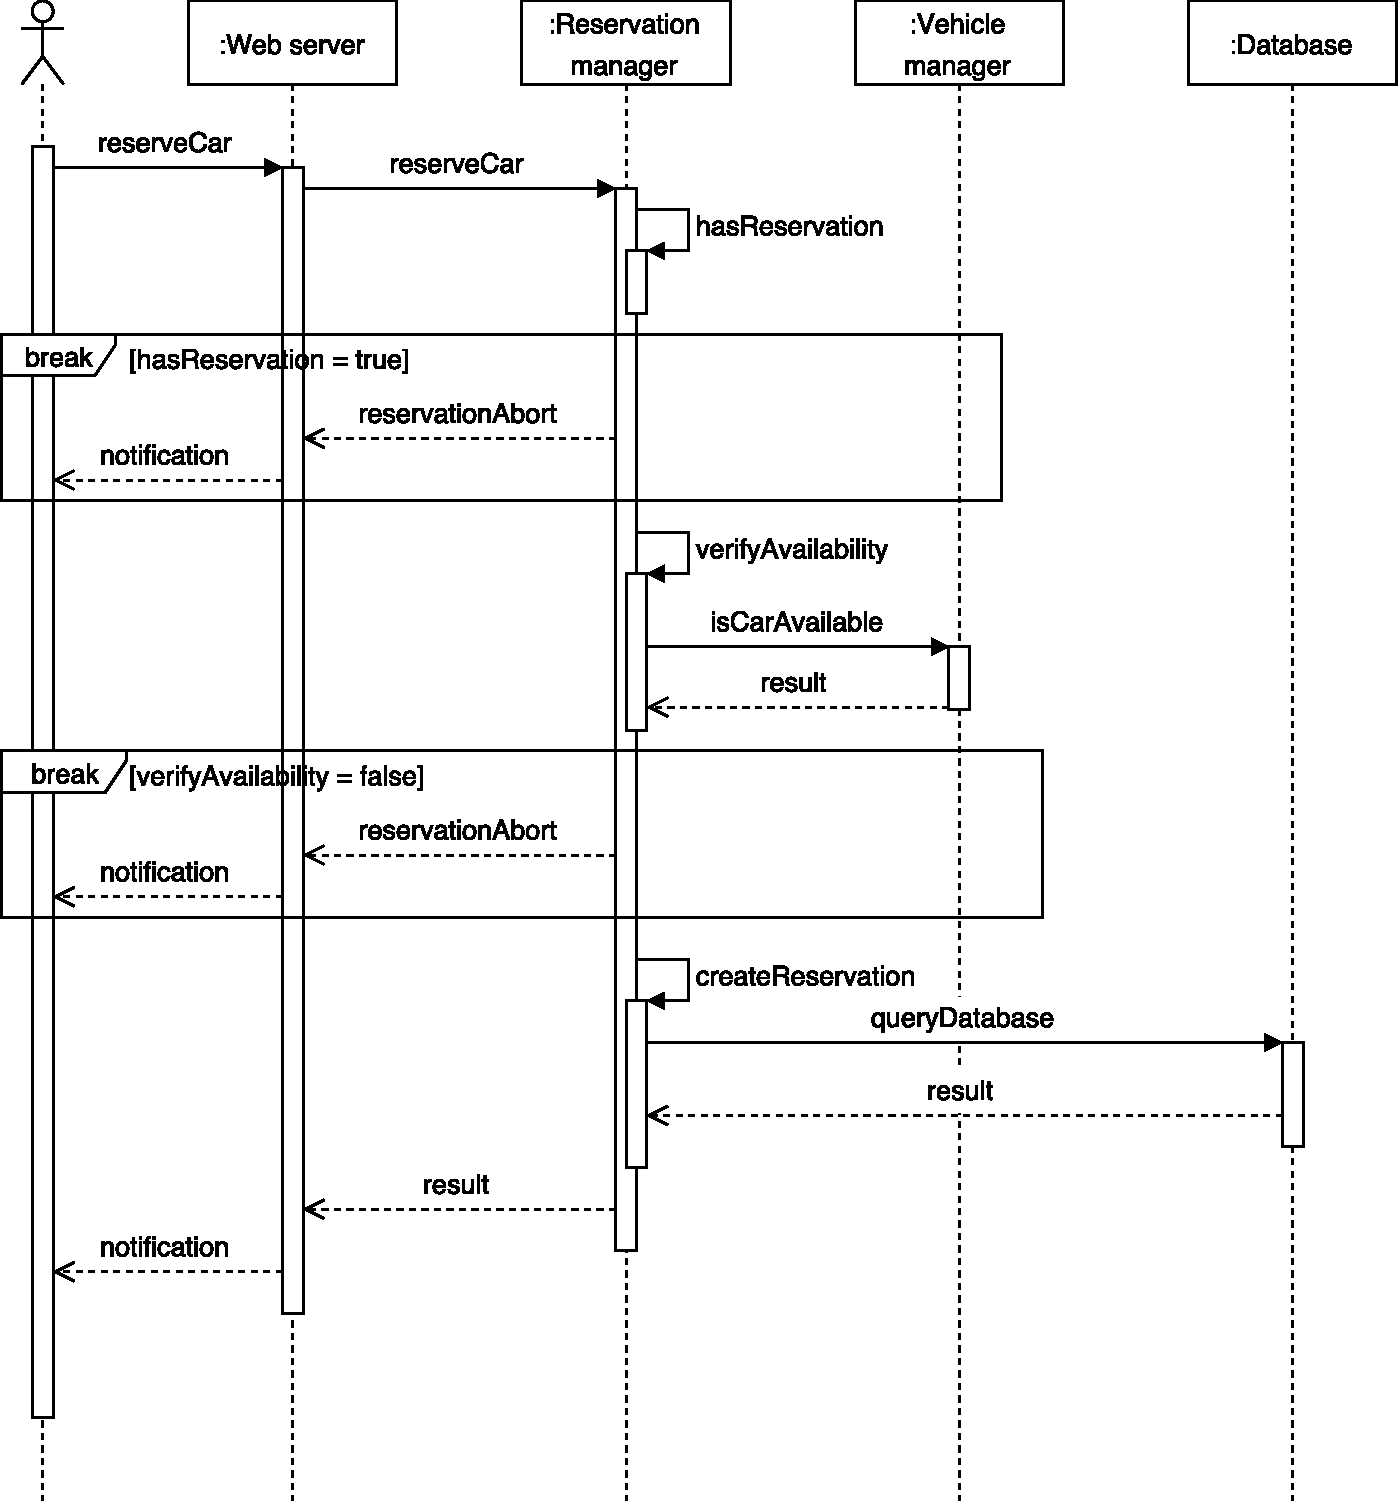
\includegraphics[width=350px]{../Datas/diagrams/reservation.pdf}
        \caption{Create reservation sequence diagram}
        \label{fig:reservation-seq-dig}
\end{figure}

\begin{figure}[H]
	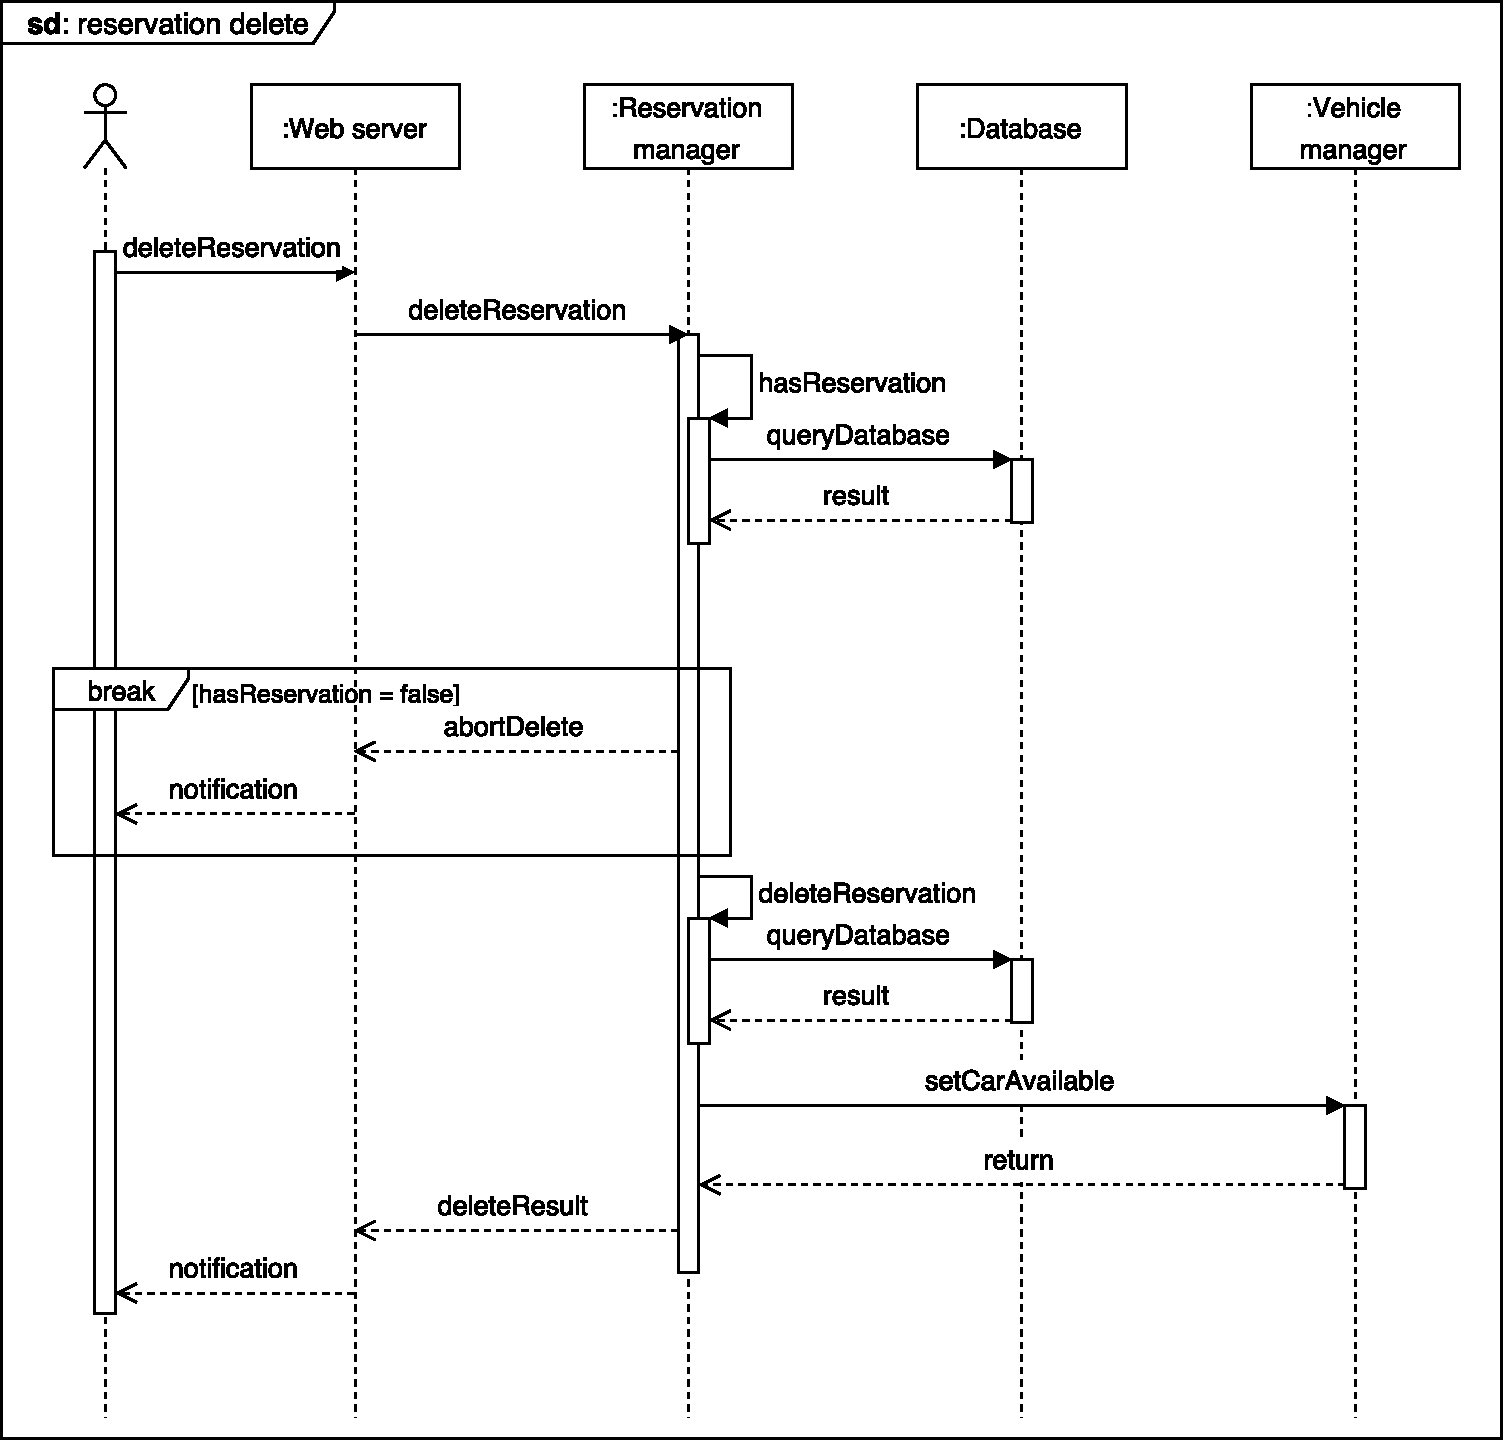
\includegraphics[width=350px]{../Datas/diagrams/res-del.pdf}
	\caption{Delete reservation sequence diagram}
	\label{fig:del-res}
\end{figure}

\begin{figure}[H]
        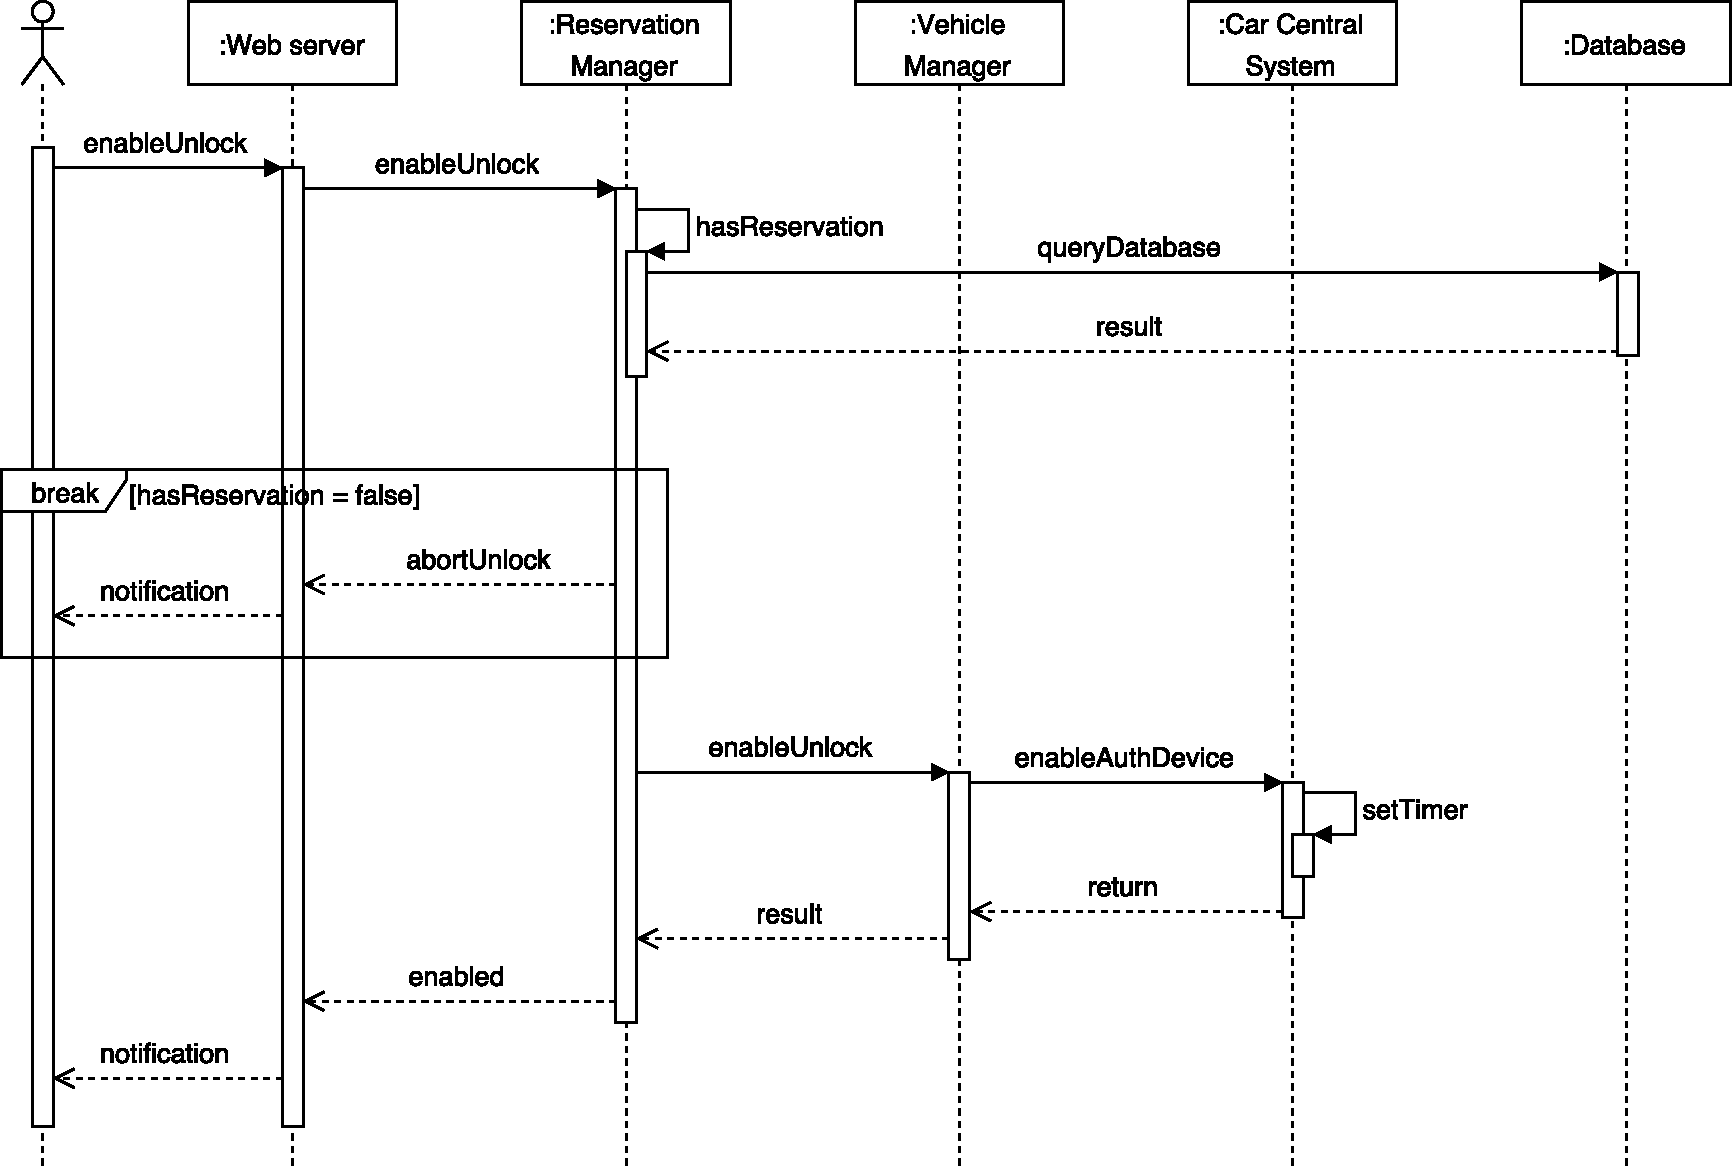
\includegraphics[width=350px]{../Datas/diagrams/unlock.pdf}
        \caption{Enable unlock sequence diagram}
        \label{fig:unlock-pt1-seq-dig}
\end{figure}

\begin{figure}[H]
        \includegraphics[width=350px]{../Datas/diagrams/"unlock pt2".pdf}
        \caption{Unlock vehicle sequence diagram}
        \label{fig:unlock-pt2-seq-dig}
\end{figure}

\begin{figure}[H]
        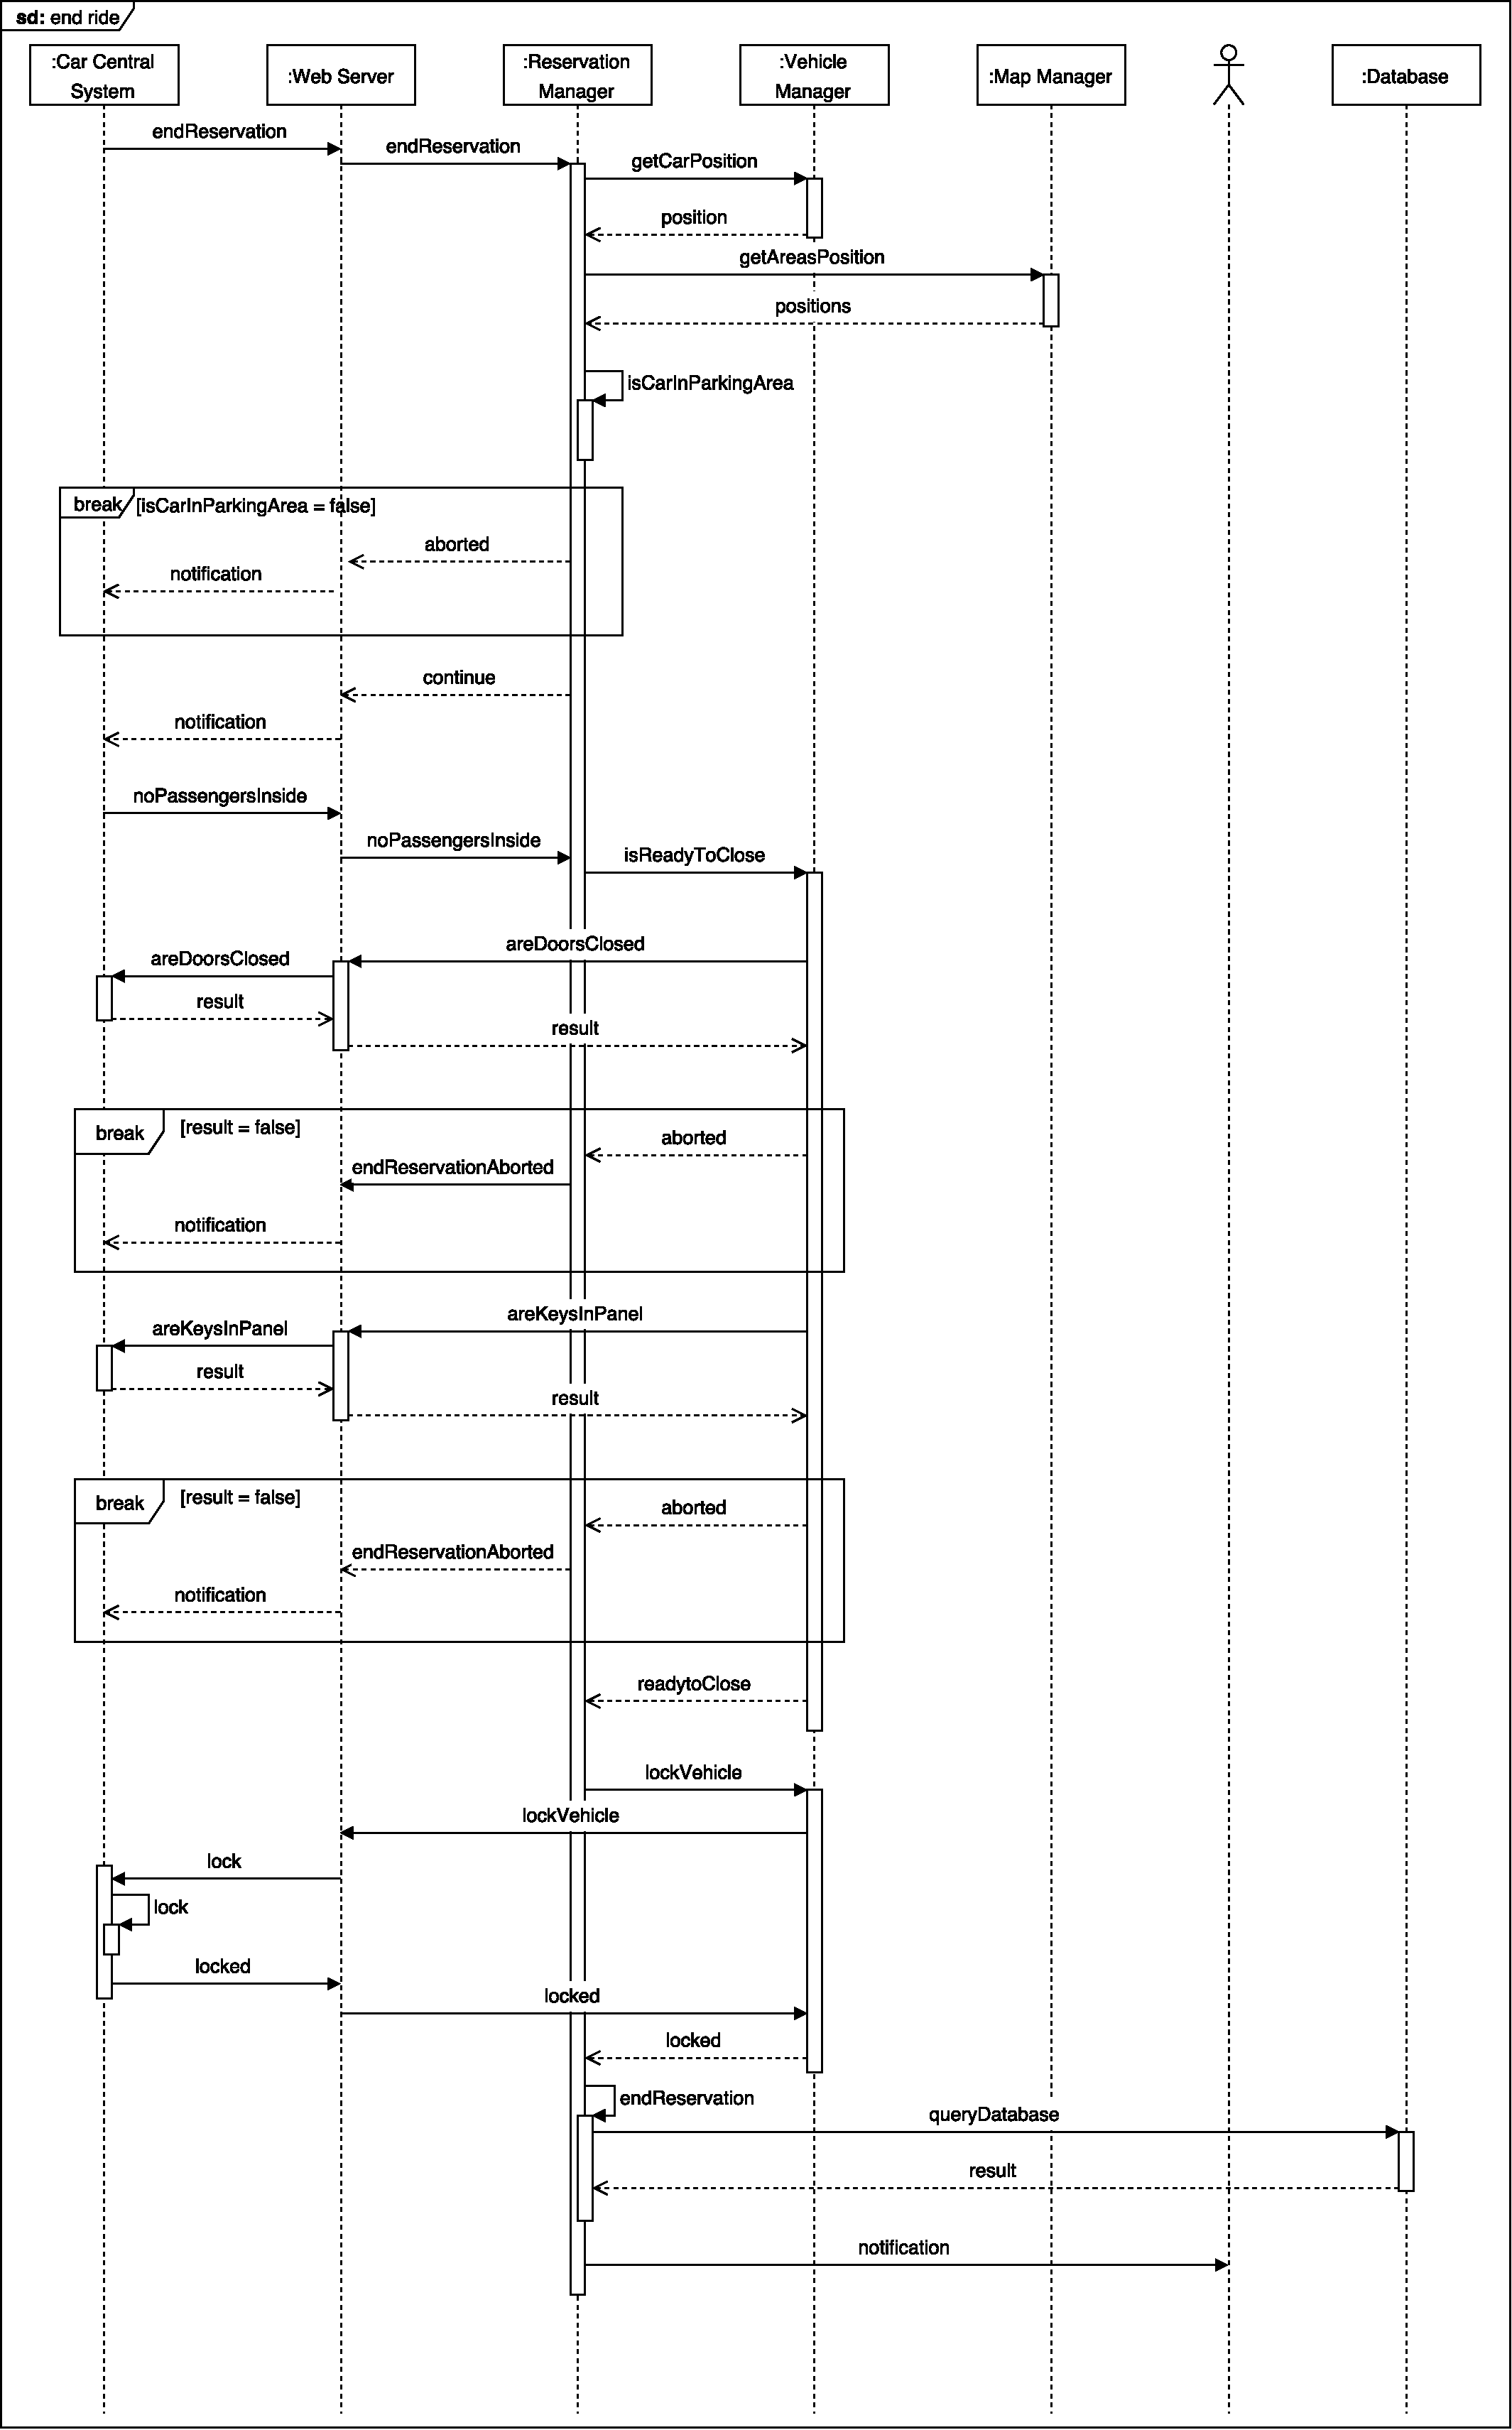
\includegraphics[width=350px]{../Datas/diagrams/endRide.pdf}
        \caption{End reservation sequence diagram}
        \label{fig:end-reserv-seq-dig}
\end{figure}
